\documentclass{article}

\usepackage{amsmath, amsfonts}
\usepackage{float}
\usepackage{geometry}
\usepackage{graphicx}
\usepackage[table]{xcolor}
\usepackage{tikz}
\usetikzlibrary{matrix}
\usepackage{algorithm}
\usepackage{algpseudocode}
\usepackage{multicol}
\usepackage [english]{babel}
\usepackage [autostyle, english = american]{csquotes}
\MakeOuterQuote{"}
%\usepackage{draftwatermark}
%\SetWatermarkText{\textsc{Draft}}
%\SetWatermarkScale{6}

\newgeometry{margin=1.25in}

\newcommand{\set}[1]{\lbrace #1 \rbrace}
\newcommand{\boundedBy}[1]{\mathcal{O} \left ( #1 \right )}
\newcommand{\expected}[1]{\mathbb{E} \left ( #1 \right )}
\newcommand{\exprv}[1]{\text{Exp} \left( #1 \right )}
\newcommand{\uniformrv}[2]{\mathcal{U} \left( #1, #2 \right )}
\newcommand{\FuncCall}[2]{\textsc{#1} \left ( #2 \right )}
\newcommand{\prob}[1]{\mathbb{P}\left(#1\right)}
\newcommand{\cprob}[2]{\prob{#1\lvert#2}}
\newcommand{\factcheck}[0]{\textcolor{red}{VERIFY}}
\newcommand{\eqn}[1]{\ref{eqn:#1}}

\begin{document}

\author{Garrett Lewellen}
\title{GPU Accelerated Expectation Maximization for Gaussian Mixture Models using CUDA}

\maketitle

\section{Introduction}

Gaussian Mixture Models \cite[435-439]{bishop2006} offer a simple way to capture complex densities by employing a linear combination of $K$ multivariate normal distributions, each with their own mean, covariance, and mixture coefficient, $\pi_{k}$, s.t. $\sum_{k} \pi_{k} = 1$.

\begin{equation}
	p( x ) = \sum_{k = 1}^{K} \pi_{k} p(x \lvert \mu_k, \Sigma_k)
\end{equation}

Of practical interest is the learning of the number of components and the values of the parameters. Evaluation criteria, such as Akaike and Bayesian, can be used to identify the number of components, or non-parametric models like Dirichlet processes can be used to avoid the matter all together. We won't cover these techniques here, but will instead focus on finding the values of the parameters given sufficient training data using the Expectation-Maximization algorithm \cite{dempster1977maximum}, and doing so efficiently on the GPU. Technical considerations will be discussed and the work will conclude with an empirical evaluation of sequential and parallel implementations for the CPU, and a massively parallel implementation for the GPU for varying numbers of components, points, and point dimensions.

\section{Multivariate Normal Distribution}

The multivariate normal distribution With mean, $\mu \in \mathbb{R}^d, d \in \mathbb{N}_1$, and symmetric, positive definite covariance, $\Sigma \in \mathbb{R}^{d \times d}$, is given by:

\begin{equation}
	p( x \lvert \mu, \Sigma ) = \frac{1}{\sqrt{(2\pi)^d \lvert \Sigma \rvert }} \exp{\left( - (x - \mu)^{T} \Sigma^{-} (x - \mu) / 2 \right)}
	\label{eqn:mvn}
\end{equation}

From a computational perspective, we will be interested in evaluating the density for $N$ values. Thus, a naive implementation would be bounded by $\boundedBy{N d^4}$ due to the matrix determinate in the normalization term. We can improve upon this by computing the Cholesky factorization, $\Sigma = L L^T$, where $L$ is a lower triangular matrix \cite[157-158]{kincaid2002}. The factorization requires $\boundedBy{d^3}$ time and computing the determinate becomes $\boundedBy{d}$ by taking advantage of the fact that $\det\left(L L^T\right) = \det(L)^2 = \prod_i L_{i,i}^2$. Further, we can precompute the factorization and normalization factor for a given parameterization which leaves us with complexity of the Mahalanobis distance given by the quadratic form in the exponential. Naive computation requires one perform two vector matrix operations and find the inverse of the covariance matrix with worst case behavior $\boundedBy{d^3}$. Leveraging the Cholesky factorization, we'll end up solving a series of triangular systems by forward and backward substitution in $\boundedBy{d^2}$ and completing an inner product in $\boundedBy{d}$ as given by $L z = x - \mu$, $L^T z = y$, and $(x-\mu)^T y$. Thus, our pre-initialization time is $\boundedBy{d^3}$ and density determination given by $\boundedBy{N d^2}$. Further optimizations are possible by considering special diagonal cases of the covariance matrix, such as the isotropic, $\Sigma = \sigma I$, and non-isotropic, $\Sigma_{k,k} = \sigma_k$, configurations. For robustness, we'll stick with the full covariance.

\begin{equation}
	\log p( x \lvert \mu, \Sigma ) = - \frac{1}{2} \left( d \log 2\pi + \log \lvert \Sigma \rvert \right ) - \frac{1}{2} (x - \mu)^{T} \Sigma^{-} (x - \mu)
\end{equation}

To avoid numerical issues such as overflow and underflow, we're going to consider $\log p(x \lvert \mu, \Sigma)$ throughout the remainder of the work. For estimates of the covariance matrix, we will want more samples than the dimension of the data to avoid a singular covariance matrix \cite{fan2016overview}. Even with this criteria satisfied, it may still be possible to produce a singular matrix if some of the data are collinear and span a subspace of $\mathbb{R}^d$.

\section{Expectation Maximization}

From an unsupervised learning point of view, GMMs can be seen as a generalization of k-means allowing for partial assignment of points to multiple classes. A possible classifier is given by $k^{*} = \arg\max_k \, \log \pi_{k} + \log p(x \lvert \mu_k, \Sigma_k)$. Alternatively, multiple components can be used to represent a single class and we argmax over the corresponding subset sums. The utility of of GMMs goes beyond classification, and can be used for regression as well. The Expectation-Maximization (EM) algorithm will be used to find the parameters of of the model by starting with an initial guess for the parameters given by uniform mixing coefficients, means determined by the k-means algorithm, and spherical covariances for each component. Then, the algorithm iteratively computes probabilities given a fixed set of parameters, then updating those parameters by maximizing the log-likelihood of the data:

\begin{equation}
	\mathcal{L} \left( \mathcal{D} \lvert \mu, \Sigma \right) = \sum_{n = 1}^{N} \log p(x_n) = \sum_{n=1}^{N} \log{ \left [ \sum_{k = 1}^{K} \pi_{k} p \left( x_n \lvert \mu_k, \Sigma_k \right ) \right ] }
	\label{eqn:loglikelihood}
\end{equation}

Because we are dealing with exponents and logarithms, it's very easy to end up with underflow and overflow situations, so we'll continue the trend of working in log-space and also make use of the "log-sum-exp trick" to avoid these complications:

\begin{equation}
	\log p( x ) = a + \log \left[ \sum_{k = 1}^{K} \exp{ \left( \log \pi_{k} + \log p(x \lvert \mu_k, \Sigma_k) - a \right ) } \right ]
\end{equation}

Where the $a$ term is the maximum exponential argument within a stated sum. Within the expectation stage of the algorithm we will compute the posterior distributions of the components conditioned on the training data (we omit the mixing coefficient since it cancels out in the maximization steps of $\mu_k$ and $\Sigma_k$, and account for it explicitly in the update of $\pi_k$):

\begin{equation}
	\gamma_{k, n} = \frac{ p \left ( x_n \lvert \mu_k, \Sigma_k \right ) }{ p(x) } \qquad \Gamma_k = \sum_{n=1}^{N} \gamma_{k, n}
\end{equation}

\begin{equation}
	\log \gamma_{k, n} =  \log p \left ( x_n \lvert \mu_k, \Sigma_k \right )  - \log p(x) \qquad \log \Gamma_k = a + \log \left [ \sum_{n=1}^{N} \exp{ \left( \log \gamma_{k, n} - a \right )} \right ]
\end{equation}

The new parameters are resolved within the maximization step:

\begin{equation}
	\pi_{k}^{(t+1)} = \frac{ \pi_{k}^{(t)} \Gamma_k }{ \sum_{i=1}^{K} \pi_{i}^{(t)} \Gamma_i }
	\qquad
	\log \pi_{k}^{(t+1)} = \log \pi_{k}^{(t)} + \log \Gamma_k - a - \log \left [ \sum_{i=1}^{K} \exp{ \left( \log \pi_{i}^{(t)} + \log \Gamma_i - a \right )} \right ]
\end{equation}

\begin{equation}
	\mu_k^{(t+1)} = \frac{ \sum_{n=1}^{N} x_n \gamma_{n, k} }{ \Gamma_k  }
	\qquad
	\mu_k^{(t+1)} = \frac{ \sum_{n=1}^{N} x_n \exp{ \log \gamma_{n, k} } }{ \exp{ \log \Gamma_k }  }
\end{equation}

\begin{equation}
	\Sigma_k^{(t+1)} = \frac{ \sum_{n=1}^{N} (x_n - \mu_k^{(t+1)}) (x_n - \mu_k^{(t+1)})^T \gamma_{n, k} }{ \Gamma_k  }
\end{equation}

\begin{equation}
	\Sigma_k^{(t+1)} = \frac{ \sum_{n=1}^{N} (x_n - \mu_k^{(t+1)}) (x_n - \mu_k^{(t+1)})^T \exp \log \gamma_{n, k} }{ \exp \log \Gamma_k  }
\end{equation}

The algorithm continues back and forth between expectation and maximization stages until the change in log likelihood is less than some epsilon, or a maximum number of user specified iterations has elapsed.

\section{Implementations}

\paragraph{Sequential} Per iteration complexity given by $\boundedBy{2 K N d^2 + K N d + 2K + N + K d^3}$. We expect $d \le K < N$ because too many dimensions leads to a lot of dead space and too many components results in overfitting of the data. Thus, the dominating term for sequential execution is given by $\boundedBy{ 2 K N d^2 }$. 

\paragraph{Parallel} There are two natural data parallelisms that appear in the algorithm. The calculation of the $\mathcal{L}$ and $\gamma$ across points, while the probabilitiy densities and parameter updates have natural parallelisms across components. Each POSIX thread runs the full iterative algorithm with individual stages coordinated by barrier synchronization. Resulting complexity is given by $\mathcal{O}\left(\frac{2}{P} d^2 K N \right)$ for work coordinated across $P$ processors.


\begin{figure}[H]
	\resizebox{\linewidth}{!}{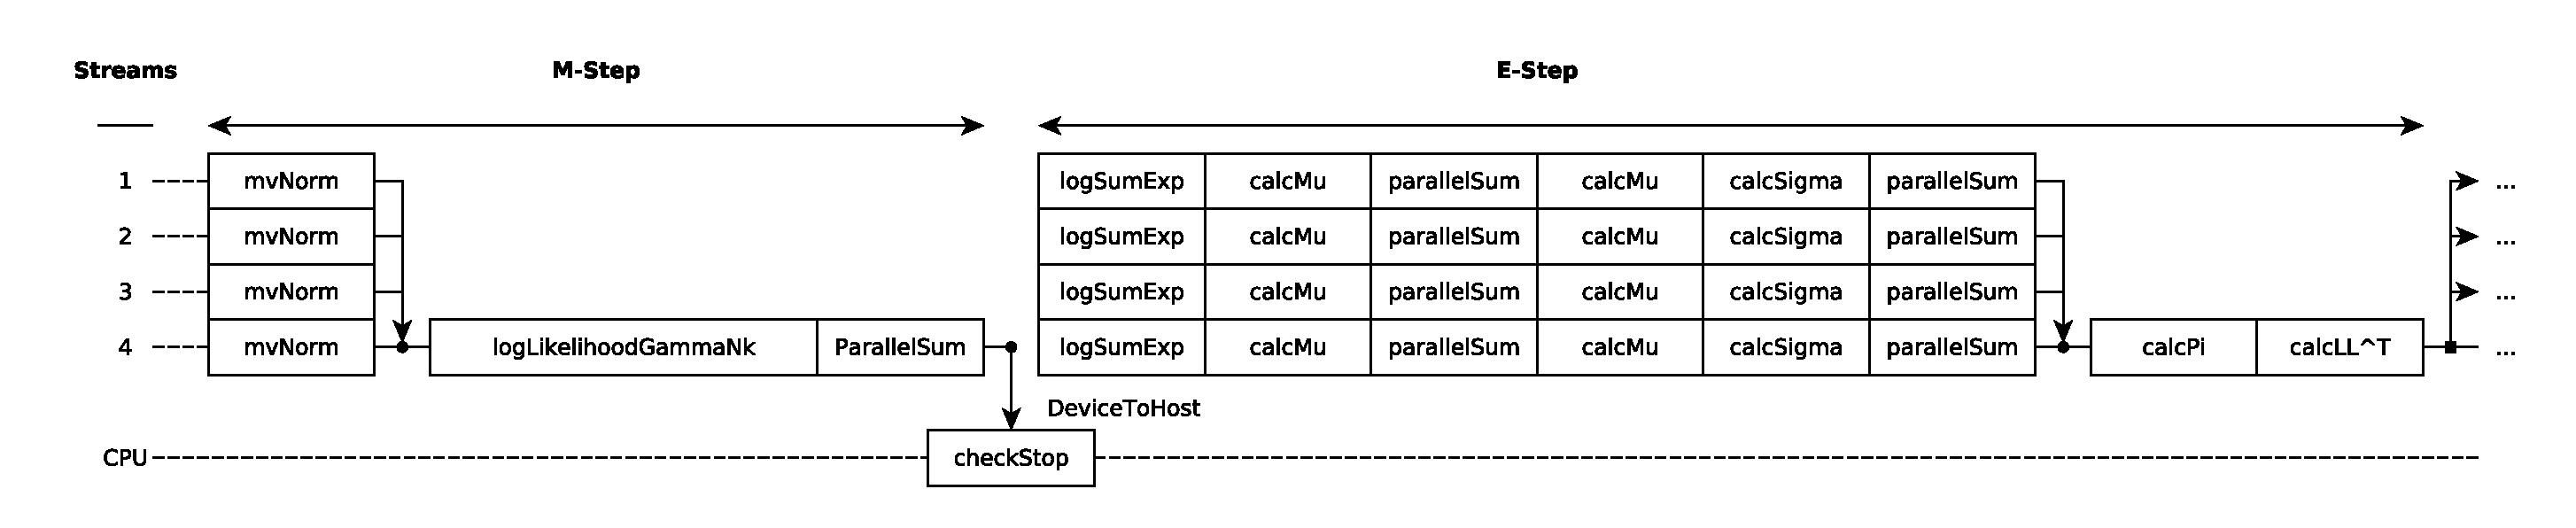
\includegraphics{doc/cudaFlow.eps}}
	\caption{Execution of the EM-Algorithm on the GPU using the CUDA programming model. Synchronization junctions denoted in black.}
\end{figure}

\paragraph{Massively Parallel} The parallel implementation can be taken and mapped over to the GPU with parallelism taken across points and components depending on the terms being computed. There are several types of parallelism that we will leverage under the CUDA programming model. For the calculation of $\log p\left(x | \mu_k, \Sigma_k \right)$ we compute each point in parallel by forming a grid of one dimensional blocks, and use streams with event synchronization to carry out each component in parallel across the streaming multiprocessors. Calculation of the loglikelihood and $\log \gamma_{n,k}$ is done by computing and storing $\log p(x)$, then updating the storage for $\log p\left(x|\mu_k,\Sigma_k\right)$, and then performing a parallel reduction over $\log p(x)$ to produce the loglikelihood. Parallel reductions are a core tasks are implemented by first standardizing the input array of points to an supremum power of two, then reducing each block using shared memory, and applying a linear map to the memory so that successive block reductions can be applied. Several additional approaches are discussed in \cite{harris2007optimizing}. Once the loglikelihood is computed, the streams are synchronized with the host and the result is copied from the device back to the host. To compute $\log \Gamma_k$, $\log \gamma_{n,k}$ is copied to a working memory and a maximum parallel reduction is performed. The resulting maximum is used in a separate exponential map for numerical stability when computing the parallel reduction of each component to yield $\log \Gamma_k$. Updates to the mean and covariances are performed by mapping each term to a working memory allocated for each component's stream and executing a parallel reduction to yield the updated mean and covariance. Once all component streams have been synchronized, the mixture coefficients and Cholesky decompositions of the covariances is computed with a single kernel invocation parallel in the number of components.

The main design consideration was whether or not use streams. For larger numbers of components, this will result in improved runtime performance, however, it comes at the cost of increased memory usage which limits the size of problems an end user can study with the implementation. Because the primary design goal is performance, the increase in memory was favorable to using less memory and executing each component sequentially.

To optimize the runtime of the implementation \texttt{nvprof} along with the NVIDIA Visual Profiler was used to identify performance bottlenecks. The original implementation was a naive port of the parallel C code which required frequent memory transfers between host and device resulting in significant CUDA API overhead that dominated the runtime. By transferring and allocating memory on the device beforehand, this allowed the implementation to execute primarily on the GPU and eliminate the API overhead. The second primary optimization was using streams and events for parallelization of the component probability densities and parameter updates in the maximization step. In doing so, this allowed for a $K$ fold reduction since the components calculations would be performed in parallel. The next optimization step was to streamline the parallel reductions by using block reductions against fast shared block memory minimizing the number of global memory writes instead of performing iterated reductions against sequential addressing that preformed global memory reads and writes for each point. The final optimization step was to used pinned host memory to enable zero-copy transfers from DRAM to the GPU over DMA. 

\section{Evaluation}

To evaluate the implementations we need a way of generating GMMs and sampling data from the resulting distributions. To sample from a standard univariate normal distribution one can use The Box-Muller transform, Zigguart method, or Ratio-of-uniforms method \cite{kinderman1977computer}. The latter is used here due to its simplicity and efficiency. Sampling from the multivariate normal distribution can by done by sampling a standard normal vector $\eta \sim \mathcal{N}(0 ,I_d)$ and computing $\mu + \Sigma^{1/2} \eta$ where $\Sigma^{1/2}$ can be computed by Eigendecomposition, $\Sigma^{1/2} = Q \Delta^{1/2} Q^{-}$, or Cholesky factorization, $\Sigma = L L^T, \Sigma^{1/2} = L$. The latter is used since it is more efficient. The GMM describes a generative process whereby we pick a component at random with probability given by its mixture coefficient and then sample the underlying $\mathcal{N}(\mu_k, \Sigma_k)$ distribution, and perform this process for the desired number of points.

The matter of generating GMMs it more interesting. Here we draw $\pi_i = X_i / \sum_{j} X_j$ for $X_i \sim \mathcal{U}(0, 1)$, alternatively, one could draw $\pi \sim \text{Dir}(\alpha)$. Means are drawn by $\mu \sim \mathcal{N}(0, a I_d)$ with $a > 1$ so that means are relatively spread out in $\mathbb{R}^{d}$. The more exciting prospect is how to sample the covariance matrix. This is where the Wishart distribution, $\Sigma \sim W(I_d, d, n)$ for $n > d - 1$, comes in handy. The Wishart distribution is a model of what the sample covariance matrix should look like given a series of $n$ $x_i \sim \mathcal{N}(0, I_d)$ vectors. Based on a $\boundedBy{d^2}$ method by \cite{odell1966numerical}, \cite{sawyer2007wishart} gives an equally efficient method for sampling $\Sigma^{1/2} = L$ by letting $L_{i,i} \sim \chi^2(n - i)$ and $L_{i,j} \sim \mathcal{N}(0, 1)$ for $0 \le i < d$ and $0 \le j < i$. 

To evaluate the performance of the different implementations, the wall clock time taken to run the algorithm on a synthetic instance was measured by varying each of the $N$, $K$, and $d$ parameters while holding the other two fixed. From an end user perspective wall clock time is preferable to the time the operating system actually devoted to the problem since wall clock time is more valuable. There will be variability in the results since each instance requires a different number of iterations for the log likelihood to converge. Tests were conducted on a Xeon 1245 v5 3.5 Ghz system with 32GB of memory and an NVIDIA GTX 1060 6GB graphics card with 1280 cores.

\begin{multicols}{2}
\begin{figure}[H]
	\centering
	\resizebox{\linewidth}{!}{\input{obj/timeNumPoints.tex}}
	\caption{Elapsed wall time with 95\% confidence interval for $K = 2^{3}$ and $d = 2^{1}$ across 15 samples.}
	\label{fig:timeNumPoints}
\end{figure}

\begin{figure}[H]
	\centering
	\resizebox{\linewidth}{!}{\input{obj/timePointDim.tex}}
	\caption{Elapsed wall time with 95\% confidence interval for $N = 2^{13}$ and $K = 2^{2}$ across 15 samples.}
	\label{fig:timePointDim}
\end{figure}

\columnbreak

\begin{figure}[H]
	\centering
	\resizebox{\linewidth}{!}{\input{obj/timeNumComponents.tex}}
	\caption{Elapsed wall time with 95\% confidence interval for $N = 2^{19} $ and $d = 2^{1}$ across 15 samples.}
	\label{fig:timeNumComponents}
\end{figure}

\begin{figure}[H]
	\centering
	\resizebox{\linewidth}{!}{\includegraphics{obj/speedup.eps}}
	\caption{Maximum speedup of parallel and CUDA approaches to sequential method observed across trials.}
	\label{fig:sppedup}
\end{figure}
\end{multicols}

Since the parameter space is relatively large Figures \ref{fig:timePointDim} - \ref{fig:timeNumComponents} look at varying one parameter will fixing the others to demonstrate the relative merits of each approach. When the number of points dominates the CUDA approach tends to be 18x faster; the Parallel approach tends to be 3x faster when the dimension is high; and CUDA is suitable when the num of components is high giving a 20x improvement relative to the sequential approach. Thus, when dealing with suitably large datasets, the CUDA based implementation is preferable delivering superior runtime performance without sacrificing quality.

It is important to note that the results obtained from the CUDA solution may differ to those the sequential and parallel approaches. This is due to nondeterministic round off errors associated with executing parallel reductions compared to sequential reductions \cite{collange2015numerical}, and differences in the handling of floating point values on the GPU \cite{whitehead2011precision}, notably, the presence of fused multiple add on NVIDIA GPUs which are more accurate than what is frequently implemented in CPU architectures. The following two synthetic data sets illustrate typical results of the three schemes:

\begin{figure}[H]
	\resizebox{\linewidth}{!}{\includegraphics{obj/n8192-d2-k32.png}}
	\caption{Comparison of results against a synthetic data set with $N = 2^{13}, d = 2^{1}, K = 2^{5}$.}
\end{figure}

\begin{figure}[H]
	\resizebox{\linewidth}{!}{\includegraphics{obj/n32768-d2-k64.png}}
	\caption{Comparison of results against a synthetic data set with $N = 2^{15}, d = 2^{1}, K = 2^{6}$.}
\end{figure}

\section{Conclusion}

This work demonstrated the utility of using NVIDIA GPUs to train Gaussian mixture models by the Expectation Maximization algorithm. Speedups as high as 20x were observed on synthetic datasets by varying the number of points, components, and data dimension while leaving the others fixed. It is believed that further speedups should be possible with additional passes, and the inclusion of metric data structures to limit which data is considered during calculations. Future work would pursue more memory efficient solutions on the GPU to allow for larger problem instance, and focus on providing higher level language bindings so that it can be better utilized in traditional data science toolchains.

\bibliographystyle{acm}
\bibliography{doc/references}

\end{document}
